
% A modified version of the homework template 
% of Theodore P. Pavlic 
% http://www.tedpavlic.com/post_homework_tex_example.php  
% Modified by Iqram Mahmud

% The document class specifies the type of document.  You  can
% change article to book or report.  (In books and reports, you
% can use \chapter in addition to \section and \subsection.)
% Change 11pt to 10pt for smaller sized type; change it to 12pt
% for larger sized type.  You can get two-column output like this:
% \documentclass[11pt,twocolumn]{article}

% "Packages" add extra capabilities to LaTeX that are not part
% of the basic system.  Here are a few that are often used.
% It doesn't hurt to include them, even if you don't use them,
% so you can leave this section alone.

\documentclass[a4paper, 11pt]{article}
\usepackage[latin1]{inputenc}    % Accept european-encoded (latin1) characters.
\usepackage{a4wide}              % Wide paper
\usepackage[parfill]{parskip}		% skip a line instead of indenting new paragraphs
\usepackage{palatino}
\usepackage{amsmath,amsfonts,amsthm,amssymb}
\usepackage{setspace}
\usepackage{fancyhdr}  % package for the headers and footers
\usepackage{lastpage}
\usepackage{extramarks}
\usepackage{chngpage}
\usepackage{soul}
\usepackage[usenames,dvipsnames]{color}
\usepackage{float,wrapfig}
\usepackage[pdftex]{graphicx}
\usepackage{ifthen}
\usepackage{listings}
\usepackage{courier}
\usepackage[mathscr]{eucal}
\usepackage{url}
\usepackage{hyperref}  

% removing box from \url links that is set by hyperref
\hypersetup{
colorlinks=false,
linkbordercolor={1 1 1}, % set to white
citebordercolor={1 1 1} % set to white
} 

% Change "article" to "report" to get rid of page number on title page
% REMOVE the % at the beginning of the next line to get a running header
% at the top of each page.  The header contains section title and page number.
% Change "headings" to "empty" to eliminate page numbering altogether.

%\pagestyle{headings}

% REMOVE the % at the beginning of the next line to get double-spaced text.
% Increase or decrease the 1.8 to get more or less space between lines.

%\renewcommand{\baselinestretch}{1.8}


% REMOVE the % at the beginning of the next line to spread arrays and
% tables out a bit more vertically (they are sort of cramped otherwise).
% (Not necessary if using double-spacing.)

%\renewcommand{\arraystretch}{1.2}



% Many lengths can be set to affect the appearance of the document.
% Lengths are specified with units of cm (centimeters), in (inches),
% or pt (points, 1pt = 1/72 inch).

% REMOVE the %'s at the start of the following two lines make the text
% on the page longer from top to bottom:

\topmargin=-0.45in      %
\evensidemargin=0in     %
\oddsidemargin=0in      %
\textwidth=6.5in        %
\textheight=9.0in       %
\headsep=0.25in         %

% Homework Specific Information
\newcommand{\hmwkTitle}{Stack \& Queue - Revisited}
\newcommand{\hmwkSubTitle}{} % No subtitle, so this will be excluded
\newcommand{\hmwkDueDate}{October 12, 2011}
\newcommand{\hmwkClass}{CSC 2101 - Tutorial 3}
\newcommand{\hmwkClassTime}{}
\newcommand{\hmwkClassInstructor}{Normaziah A. Aziz}
\newcommand{\hmwkAuthorName}{Tutor - Iqram Mahmud}


% Setup the header and footer
\pagestyle{fancy}                                                       %
\lhead{CSC 2101 - Tutorial 3}                                                 %
\chead{\hmwkTitle}  %
\rhead{\hmwkDueDate}                                                     %
\lfoot{\lastxmark}                                                      %
\cfoot{}                                                                %
\rfoot{Page\ \thepage\ of\ \protect\pageref{LastPage}}                  %
\renewcommand\headrulewidth{0.4pt}                                      %
\renewcommand\footrulewidth{0.4pt}                                      %

%%%%%%%%%%%%%%%%%%%%%%%%%%%%%%%%%%%%%%%%%%%%%%%%%%%%%%%%%%%%%
% Make title
\title{\vspace{1in}\textmd{ \hmwkClass\ \hmwkSubTitle\\ \hmwkTitle\ifthenelse{\equal{\hmwkSubTitle}{}}{}}\\\normalsize\vspace{0.1in}{Due\ on\ \hmwkDueDate}\\\vspace{0.1in}\large{\hmwkClassInstructor\ \hmwkClassTime}\vspace{2.4in}}
\date{}
\author{\textbf{\hmwkAuthorName}}
%%%%%%%%%%%%%%%%%%%%%%%%%%%%%%%%%%%%%%%%%%%%%%%%%%%%%%%%%%%%%


% REMOVE the %'s from the next three \setlength lines to get a 1-inch borders
% on a standard 8-1/2 inch wide page.  The default is a narrower strip of text.

%\setlength{\textwidth}{6.5 true in}
%\setlength{\oddsidemargin}{0 true in}
%\setlength{\evensidemargin}{0 true in}


% REMOVE the % on the next \setlength line to add some vertical space 
% between paragraphs.  The plus/minus stuff makes this a stretchly length.
% Change the 10pt part only, to whatever size you want the parskip to be.

%\setlength{\parskip}{10pt plus 2 pt minus 1 pt}


% REMOVE the % on the next line to remove the usual paragraph indentation.

%\setlength{\parindent}{0pt}


% REMOVE the next % if you are clueless enough to want a ragged right margin.

%\raggedright


% Fill in your own tile, author and date.  These are printed out
% later in the document, where it says \maketitle.  (You have to
% uncomment the \maketitle line to make this stuff appear in your
% paper.)  The \today will print the current date.

\begin{document}   % This is the beginning of the actual document contents.


% REMOVE the % on the next line to include title/author/date:

\maketitle 
\tableofcontents
\newpage

% REMOVE the %'s on the next lines and type an abstract if you want one:

%\begin{abstract}
%  \textit{Text of abstract goes here --- textit puts it in italics}
%\end{abstract}


% The rest of this file is where you type your paper.  You
% can divide it into sections and subsections, as shown.
% Remember to mark the end of each paragraph with a blank line!

% Beginning of section
\section{Converting Infix Expression to Postfix Using Stack}

\subsection{Procedure}
Given an infix expression (i.e. \verb|2*3-4/5|) we want to convert it into postfix (i.e. \verb|23*45/-|). 

\begin{itemize}

\item    Scan the Infix string from left to right.
\item    Initialise an empty stack.
\item    If the scanned character is an operand, add it to the Postfix string. If the scanned character is an operator and if the stack is empty Push the character to stack.
    \begin{itemize}
    \item If the scanned character is an operand and the stack is not empty, compare the precedence of the character with the element on top of the stack (stackTop). If stackTop has higher precedence over the scanned character Pop the stack else Push the scanned character to stack. Repeat this step as long as stack is not empty and stackTop has precedence over the character.
    Repeat this step till all the characters are scanned.
    \end{itemize}
\item (After all characters are scanned, we have to add any character that the stack may have to the Postfix string.) If stack is not empty add stackTop to Postfix string and Pop the stack. Repeat this step as long as stack is not empty.
\item    Return the Postfix string. 
\end{itemize}

\subsection{Implementation}
\begin{verbatim}
#include <iostream>
#include <cassert>
using namespace std;

class Stack {
    char a[100000];
    int limit;
    int top;

public:
    Stack() {
        top = 0;
        limit = 100000;
    }
    
    char pop() {
        assert( top > 0 );
        --top;
        return a[top];
    }

    char stackTop() {
        return a[top-1];
    }

    void push(char value) {
        a[top] = value;
        top ++;
    }
    
    bool isFull() {
        return top == limit;
    }

    bool isEmpty() {
        return top == 0;
    }
};

bool isoperator( char ch ) {
    if( ch == '+' || ch == '-' || ch == '/' || ch == '*' ) return true;
    else return false;
}

int priority( char ch ) {
    if( ch == '+' || ch == '-' ) return 1;
    if( ch == '*' || ch == '/' ) return 2;
    return -1;
}

string postfix( string in ) {
    Stack s;
    string ans = "";
    
    for(int i=0; i<in.size(); i++) {
        if( isoperator( in[i] ) ) {
            
            if( s.isEmpty() ) s.push( in[i] );
            else {
                while( !s.isEmpty() &&
                        priority( s.stackTop() ) > priority( in[i] ) ) 
                    ans += s.pop();
                s.push( in[i] );
            }
        }else ans += in[i];
    }

    while( !s.isEmpty() ) ans += s.pop();
    return ans;
}

int main() {
    string infix;
    cin >> infix;
    cout << postfix( infix ) << endl;
    return 0;
}
\end{verbatim}

\section{Evaluating a Postfix Expression Using Stack}
This is how following postfix expression is evaluated - \\
4 23 12 - 2 * +

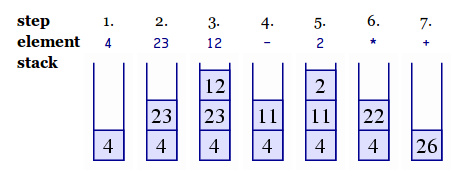
\includegraphics{image.png}


\section{Stack}
\subsection{Problem A}
Write a program that reads in a sequence of characters (that means one word) and prints them in reverse order. Use a stack.  

\subsection{Problem B}
Write a program that reads in a sequence of characters, and determines whether its parentheses "balanced." (i.e. \verb|(())| and \verb|(()()())()| are balanced, while \verb|))|, \verb|()()(| and \verb|(()()| are not)

\textbf{Hint:} for left delimiters, push onto stack; for right delimiters, pop from stack and check whether popped element matches right delimiter. 

\section{Queue}

\subsection{Problem C}
A letter means enqueue and an asterisk means dequeue in the sequence \\ 
\verb|E A S * Y * Q U E * * * S T * * * I O * N * * *| \\Write down the sequence of values returned by the dequeue operations when this sequence of operations is performed on an initially empty FIFO queue.

For this problem it's not necessary to include the code.

\section{Codes}

\begin{tabular}{|c|c|}
\hline
Infix to postfix conversion & \url{http://codepad.org/wt5qAgFV} \\ \hline
\end{tabular}

\end{document}

